\documentclass{beamer}

\usetheme[aspectratio=169]{Dresden}
\definecolor{cerulean}{rgb}{0.0, 0.48, 0.65}
%\definecolor{darkcyan}{rgb}{0.0, 0.55, 0.55}
\usecolortheme[named=cerulean]{structure}

\fontfamily{cmr}\selectfont

\usepackage{ragged2e}
\usepackage[brazilian]{babel}
\usepackage{graphicx}
\usepackage[authoryear]{natbib}
\usepackage{hyperref} 
\usepackage{subfig}
\usepackage{amssymb,amsfonts,amsmath,amsthm,euscript}
\usepackage{indentfirst}
\usepackage{ulem}
\usepackage{dsfont}
\usepackage{placeins}

\newcommand{\R}{\mathds{R}}
\newcommand{\N}{\mathds{N}}
\newcommand{\B}{\mathds{B}}
\newcommand{\Perp}{\mathcal{P}}
\newcommand{\bs}[1]{\boldsymbol{#1}}


\title{Composição Automática de Músicas utilizando Redes Neurais Recorrentes}
\author[Hahn, N. M.]{Nicolas Mathias Hahn \\ \footnotesize Orientador: Guilherme Pumi}
\institute[IME-UFRGS]{Departamento de Estatística \\ Instituto de Matemática e Estatística \\ Universidade Federal do Rio Grande do Sul (UFRGS)}
\date{Outubro de 2022 \\ \tiny Porto Alegre - RS}

\begin{document}

    \begin{frame}
        \maketitle
    \end{frame}



\section{Introdução}
    \begin{frame}{Composição Algorítmica}
        \begin{itemize}
            \justifying
            \item Composição algorítmica, ou composição automática, refere-se ao processo de criação de músicas por meio de algum processo formal com pouca ou nenhuma intervenção humana. 
            \item De acordo com \citet{maurer}, podemos encontrar três metodologias diferentes que existem em composição algorítmica: estocástica, \textit{rule-based} e inteligência artificial.
        \end{itemize}
    \end{frame}

    \begin{frame}{W. A. Mozart - \textit{Dice Music}}
        \begin{itemize}
            \justifying
            \item Wolfgang Amadeus Mozart (1756-1791) utilizou técnicas de composição algorítmica em sua obra \textit{Musikalisches Wurfelspiel} (\textit{Dice Music}).
            \item Um jogo musical que envolvia atribuir um número para fragmentos de músicas, e combiná-los ao acaso, criando uma nova peça com as partes selecionadas.
        \end{itemize}
    \end{frame}
    
    \begin{frame}{W. A. Mozart - \textit{Dice Music}}
        \centering
        \begin{figure}
            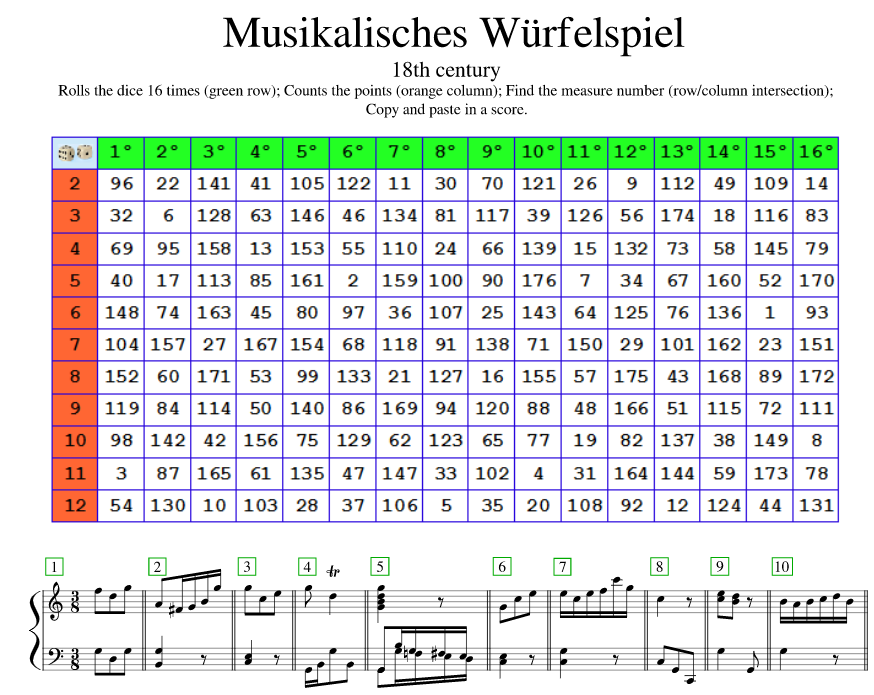
\includegraphics[scale=0.35]{figuras/dice_music.PNG}
		    \caption{\textit{Dice Music}}
		     % fonte: https://musescore.com/user/56747/scores/1742031
	    \end{figure}
    \end{frame}
    
    \begin{frame}{John Cage - \textit{Reunion}}
        \begin{itemize}
            \justifying
            \item John Cage (1912-1992), assim como Mozart, utilizou aleatoriedade em suas composições, como em \textit{Reunion}.
            \item Uma performance em que músicas são geradas ao jogar xadrez em um tabuleiro equipado com um foto receptor: cada lance emitia um som e, portanto, a música resultante é única por jogo.
        \end{itemize}
    \end{frame}

    \begin{frame}{John Cage - \textit{Reunion}}
        \centering
        \begin{figure}
            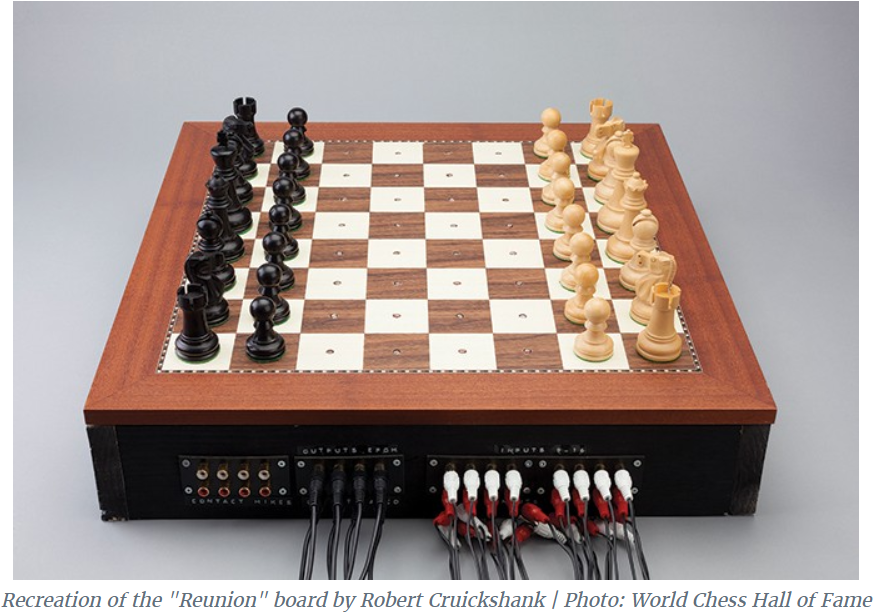
\includegraphics[scale=0.35]{figuras/reunion_board.PNG}
		    \caption{Tabuleiro de Xadrez com Foto Receptor}
		     % fonte: https://en.chessbase.com/post/50th-anniversary-of-reunion-and-the-death-of-marcel-duchamp
	    \end{figure}
    \end{frame}

    \begin{frame}{David Cope - EMI}
        \begin{itemize}
            \justifying
            \item David Cope (1941-) criou, em 1981, o EMI (\textit{Experiments in Musical Intelligence}), um sistema baseado em grandes bases de dados com descrições de estilos de diferentes estratégias composicionais.
            \item O sistema também tinha a capacidade de criar as próprias regras composicionais por meio dos novos dados recebidos.
        \end{itemize}
    \end{frame}

    \begin{frame}{David Cope - EMI}
        \centering
        \begin{figure}
            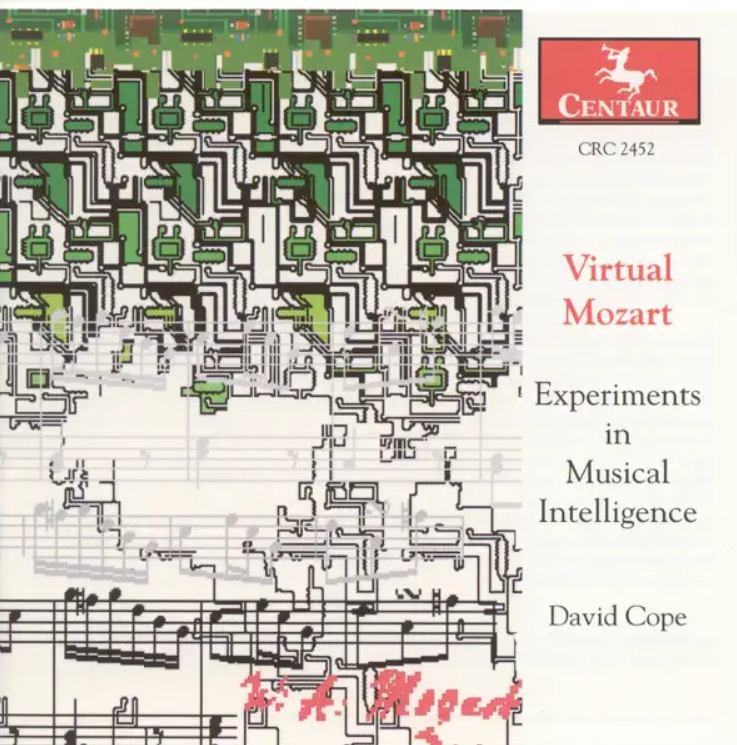
\includegraphics[scale=0.35]{figuras/emi_music.PNG}
		    \caption{Exemplo de Música feita com o EMI}
		     % fonte: https://music.apple.com/us/album/cope-d-virtual-mozart-experiments-in-musical-intelligence/341995604
	    \end{figure}
    \end{frame}

    \begin{frame}{Literatura}
        \begin{itemize}
            \justifying
            \item Via de regra, na literatura, o problema de composição musical automática é explorado com o objetivo final da composição musical em si, de forma que os modelos utilizados são ajustados para que a música gerada seja adequada em algum sentido.
            \item Detalhes técnicos como os impactos que as modificações nos parâmetros têm na composição final, ainda, são amplamente desconhecidos.
        \end{itemize}
    \end{frame}

    \begin{frame}{Objetivos}
        \begin{itemize}
            \justifying
            \item Estudar o quão sensível é um modelo de rede neural, baseado em processamento de linguagem natural, construído para composição musical.
            \item A mensuração será feita com a perplexidade, uma medida oriunda da teoria da informação.
            \item Avaliar, de forma subjetiva, as peças musicais obtidas em relação à musicalidade e qualidade.
        \end{itemize}
    \end{frame}

\section{Referencial Teórico}
    \begin{frame}{RNA - Redes Neurais Artificiais}
        \begin{itemize}
            \justifying
            \item Redes Neurais Artificiais (RNA) são técnicas de aprendizagem de máquina inspiradas no mecanismo de aprendizagem presente em organismos vivos \citep{aggarwal2018}.
            \item Nos seus primórdios, os algoritmos tinham o intuito de ser um modelo computacional capaz de imitar a aprendizagem ocorrida no cérebro \citep{goodfellow2016}.
        \end{itemize} 
    \end{frame}
   
    \begin{frame}{RNA - Neurônio}
        \centering
        \begin{figure}
            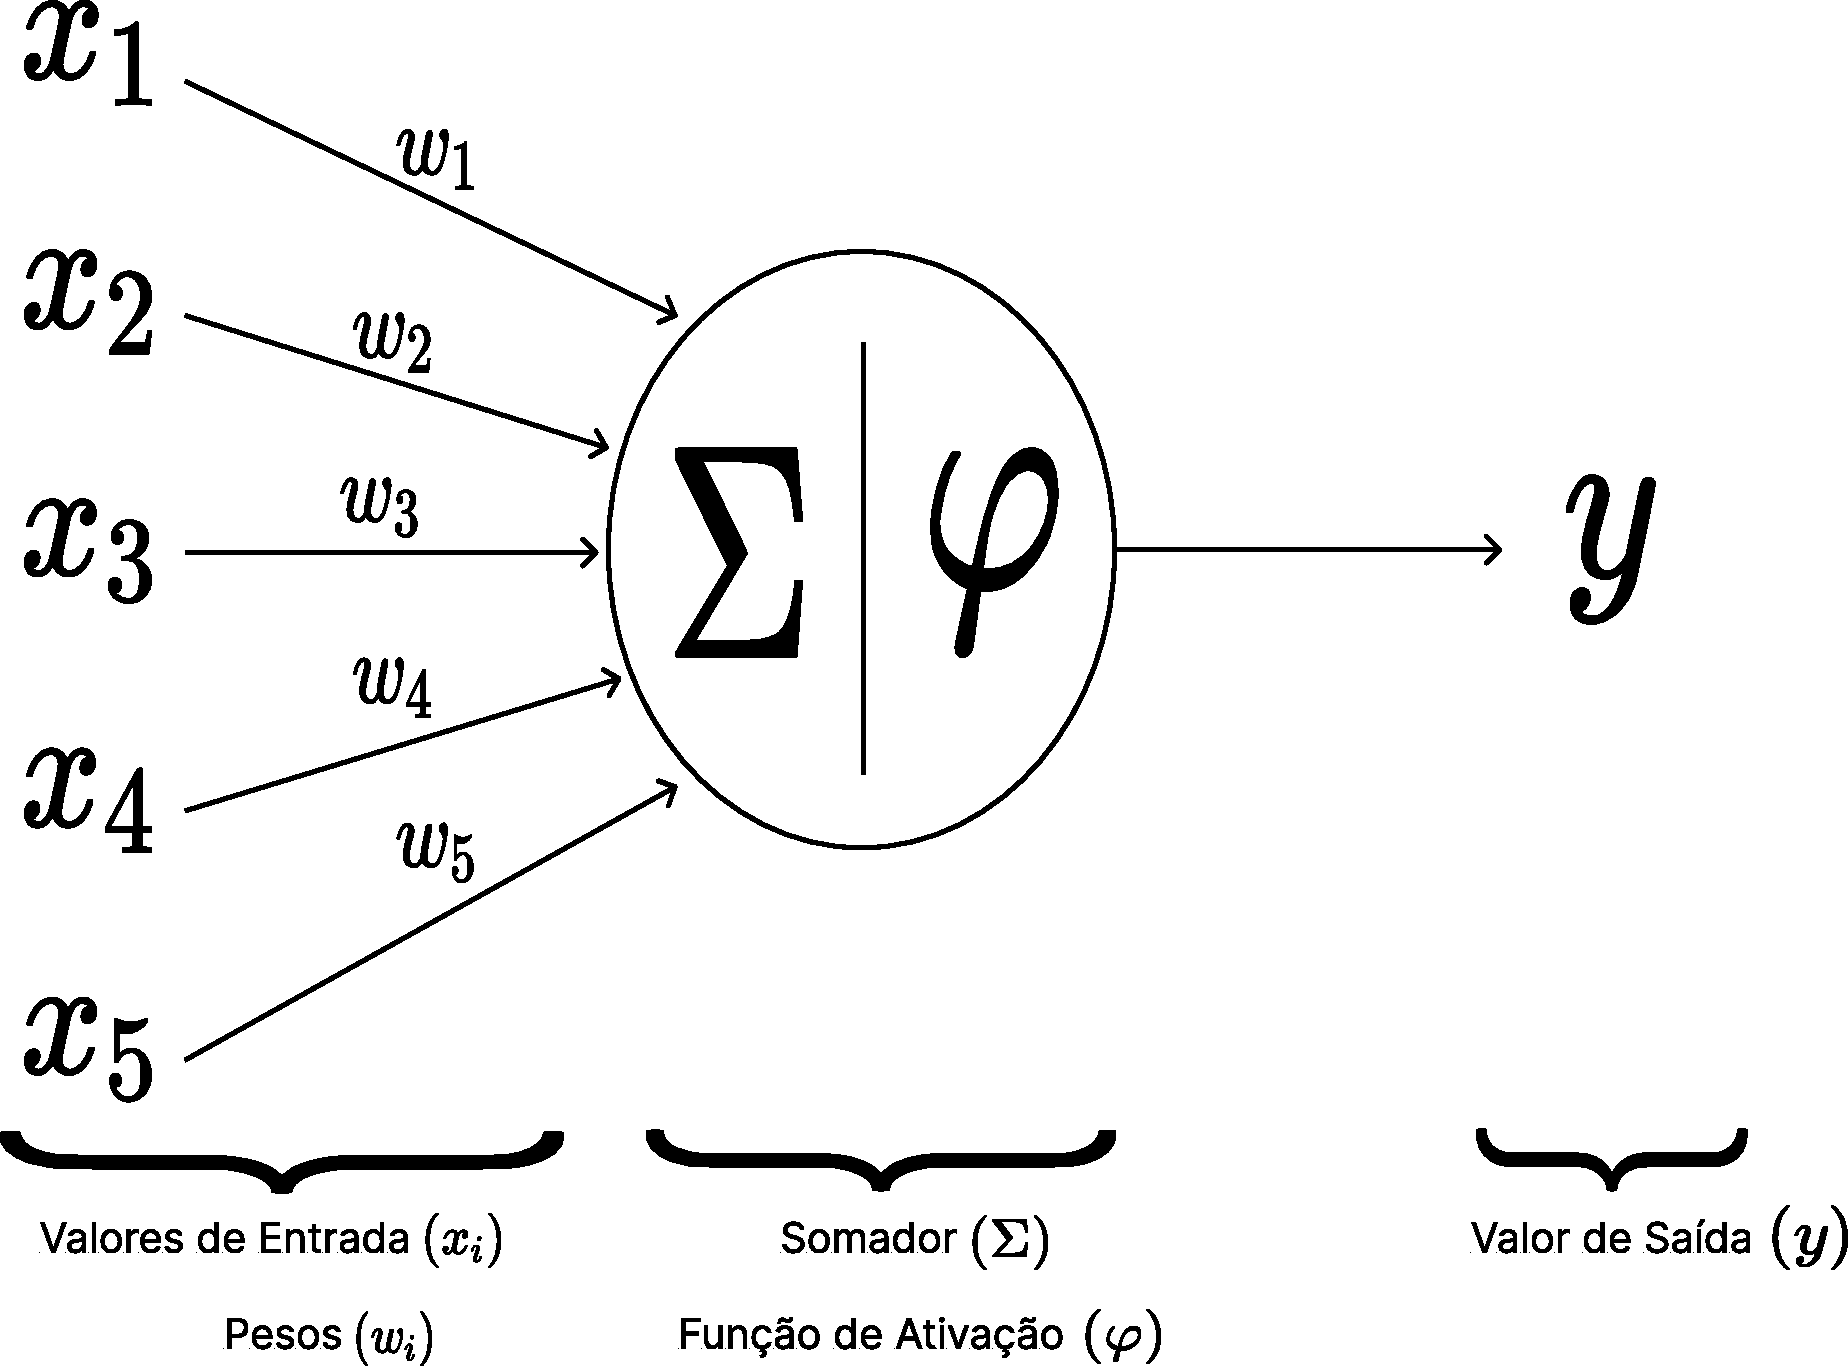
\includegraphics[scale=0.25]{figuras/neuron_model.pdf}
		    \caption{Modelo Neuronal \citep[adaptado de][]{hair2005,haykin2009}}
	    \end{figure}
    \end{frame}

    \begin{frame}{RNA - Função de Ativação}
        \begin{itemize}
            \justifying
            \item Uma função de ativação pode ser linear ou não linear. 
            \item Seu objetivo em geral é transformar o resultado de $\Sigma$ para um valor que esteja de acordo com a distribuição de $y_k$. 
            \item A escolha de uma particular função de ativação depende do problema que o neurônio almeja resolver. 
        \end{itemize}
    \end{frame}

    \begin{frame}{RNA - Função de Ativação}
    % https://tex.stackexchange.com/questions/391369/two-column-items-with-titles-in-a-beamer
        \begin{columns}[onlytextwidth,t]
            \begin{column}{0.48\textwidth}
                \centering
                \textbf{Sigmóide ou \textit{Logit}}
                
                \begin{figure}
                    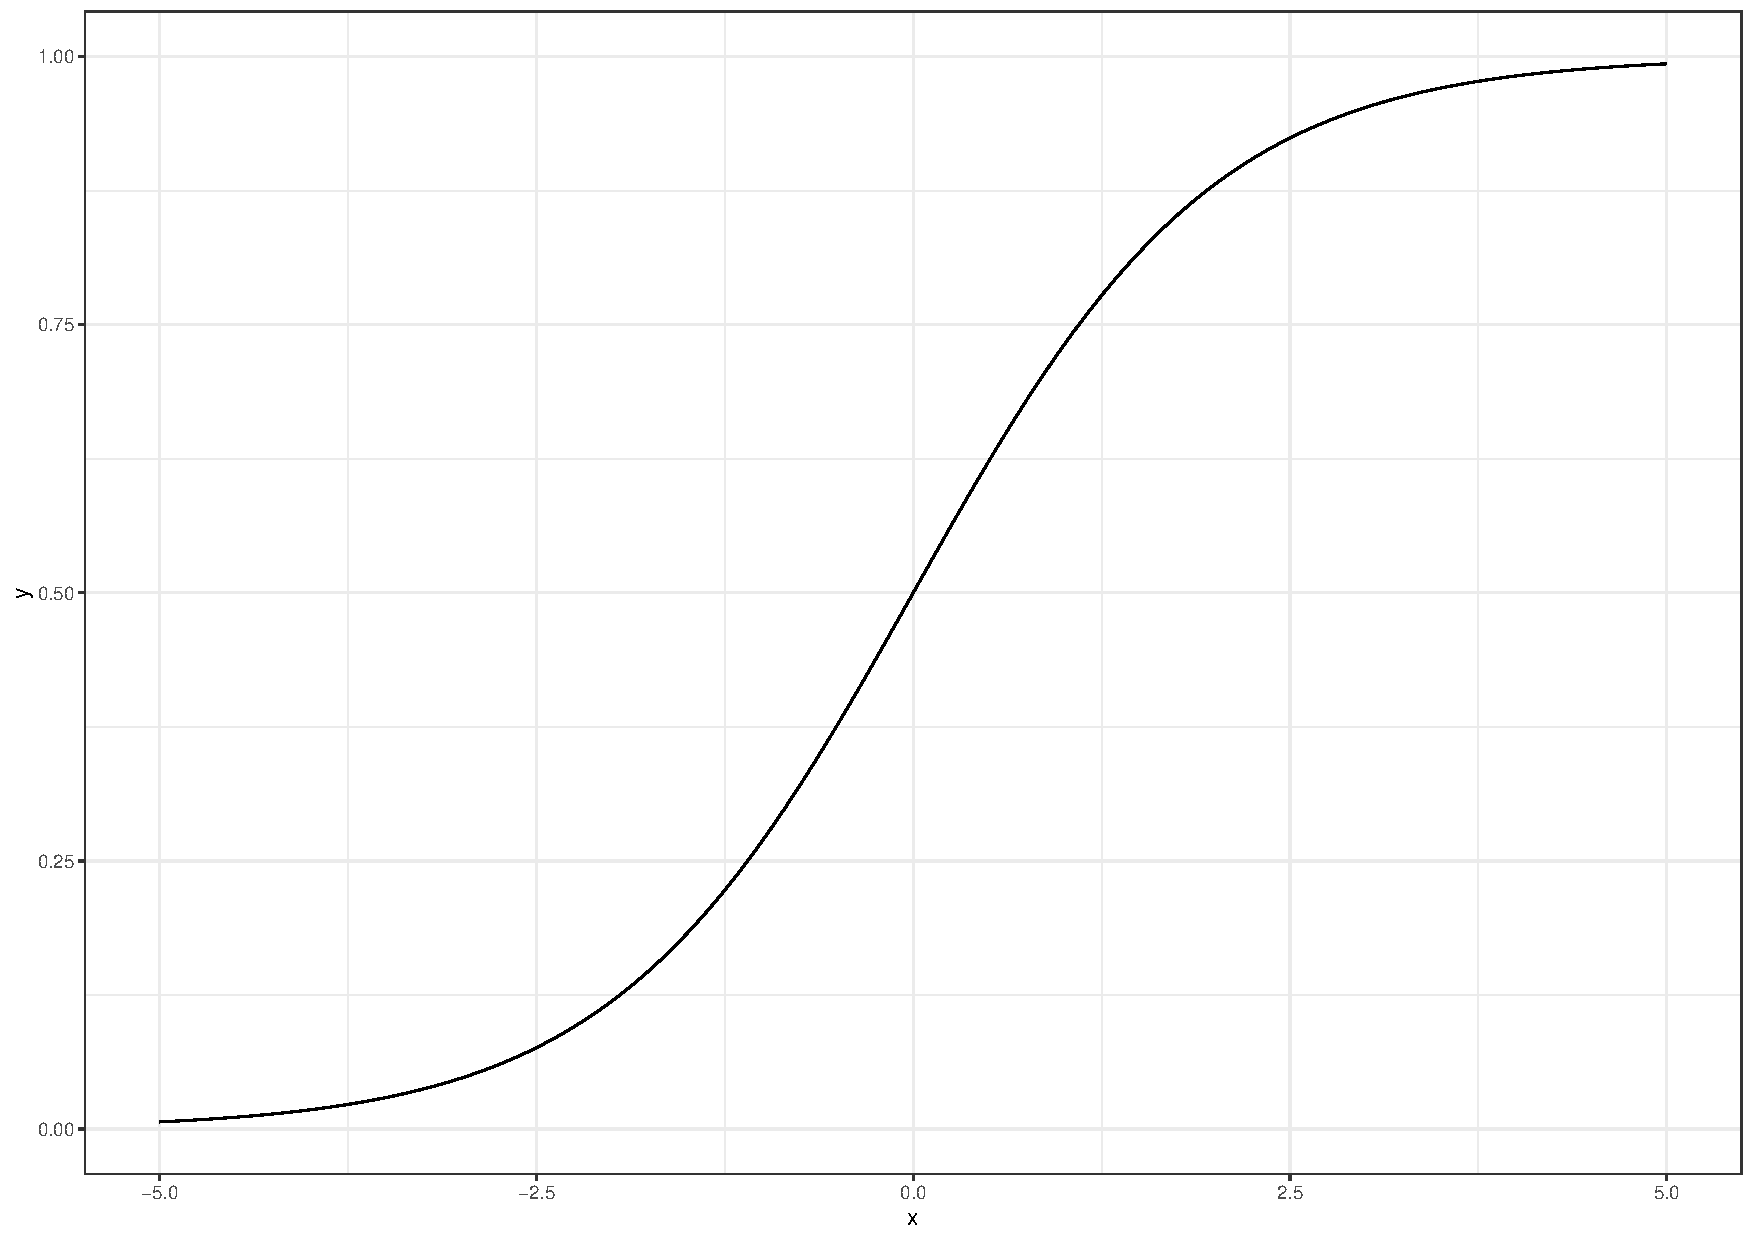
\includegraphics[scale=0.12]{figuras/sigmoid.pdf}
	            \end{figure}
	               
	            $f: \R \rightarrow (0,1)$ dada por 
	            \[f(x) := \frac{1}{1 + e^{-x}}\]
	            
            \end{column}

            \begin{column}{0.48\textwidth}
                \centering
                \textbf{Tangente Hiperbólica (\textit{tanh})}
            
                \begin{figure}
                     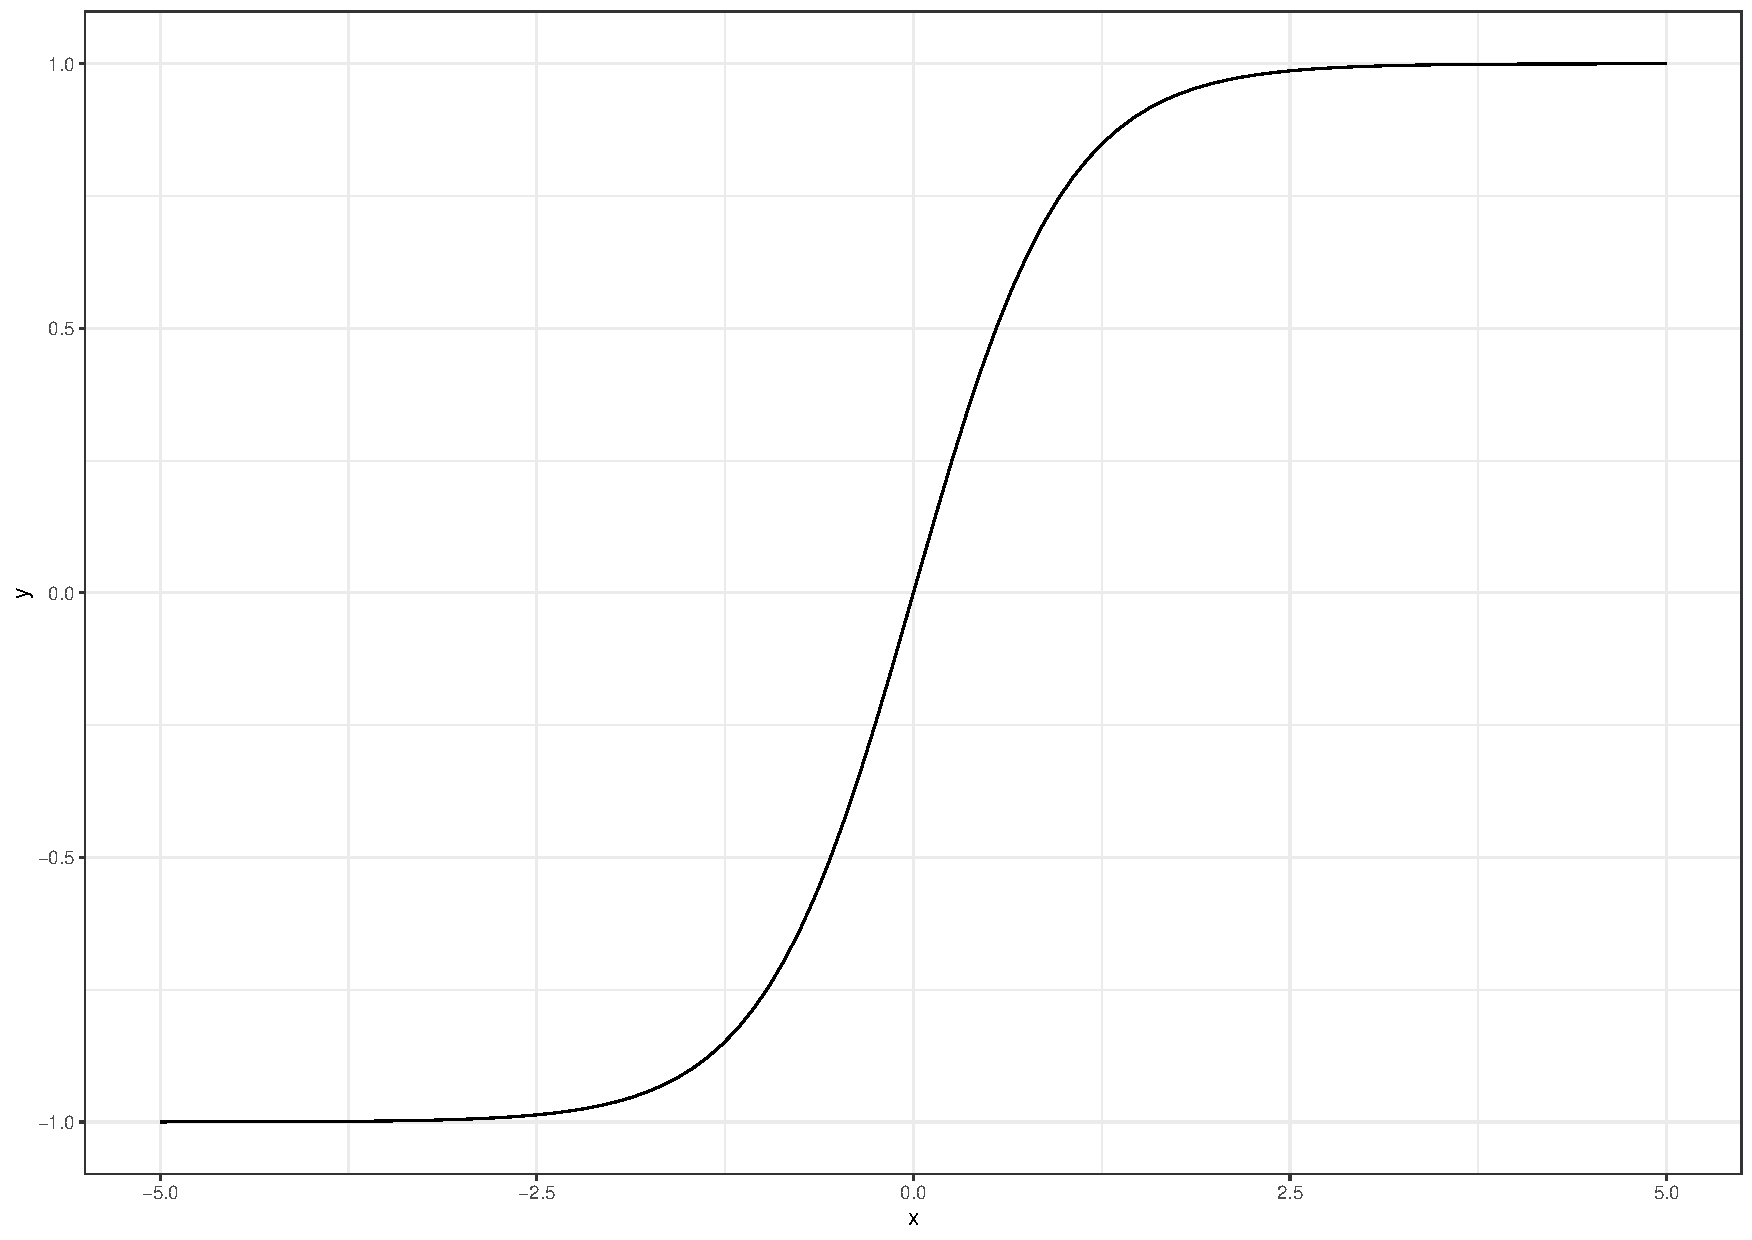
\includegraphics[scale=0.12]{figuras/tanh.pdf}
	            \end{figure}
	            
	            $f:\R \rightarrow (-1,1)$ dada por 
                \[f(x) := \frac{e^{x}-e^{-x}}{e^{x}+e^{-x}}\]
 
            \end{column}
        \end{columns}
    \end{frame}

    \begin{frame}{RNA - Arquitetura}
        \begin{itemize}
            \justifying
            \item \textbf{entrada:} constituída por nós de fonte, em que cada nó representa uma variável independente. 
            \item \textbf{saída:} composta por neurônios, com a diferença que seu valor de saída é definitivo. No caso de um modelo preditivo, o valor será o resultado da previsão.
            \item \textbf{intermediária ou oculta:} assim como a camada de saída, é composta por neurônios. Seus valores de entrada podem ser originados da camada de entrada ou da camada oculta anterior, bem como seus valores de saída podem alimentar a próxima camada oculta ou a camada de saída.
        \end{itemize}
    \end{frame}
    
    \begin{frame}{RNA - Arquitetura}
        \centering
        \begin{figure}
            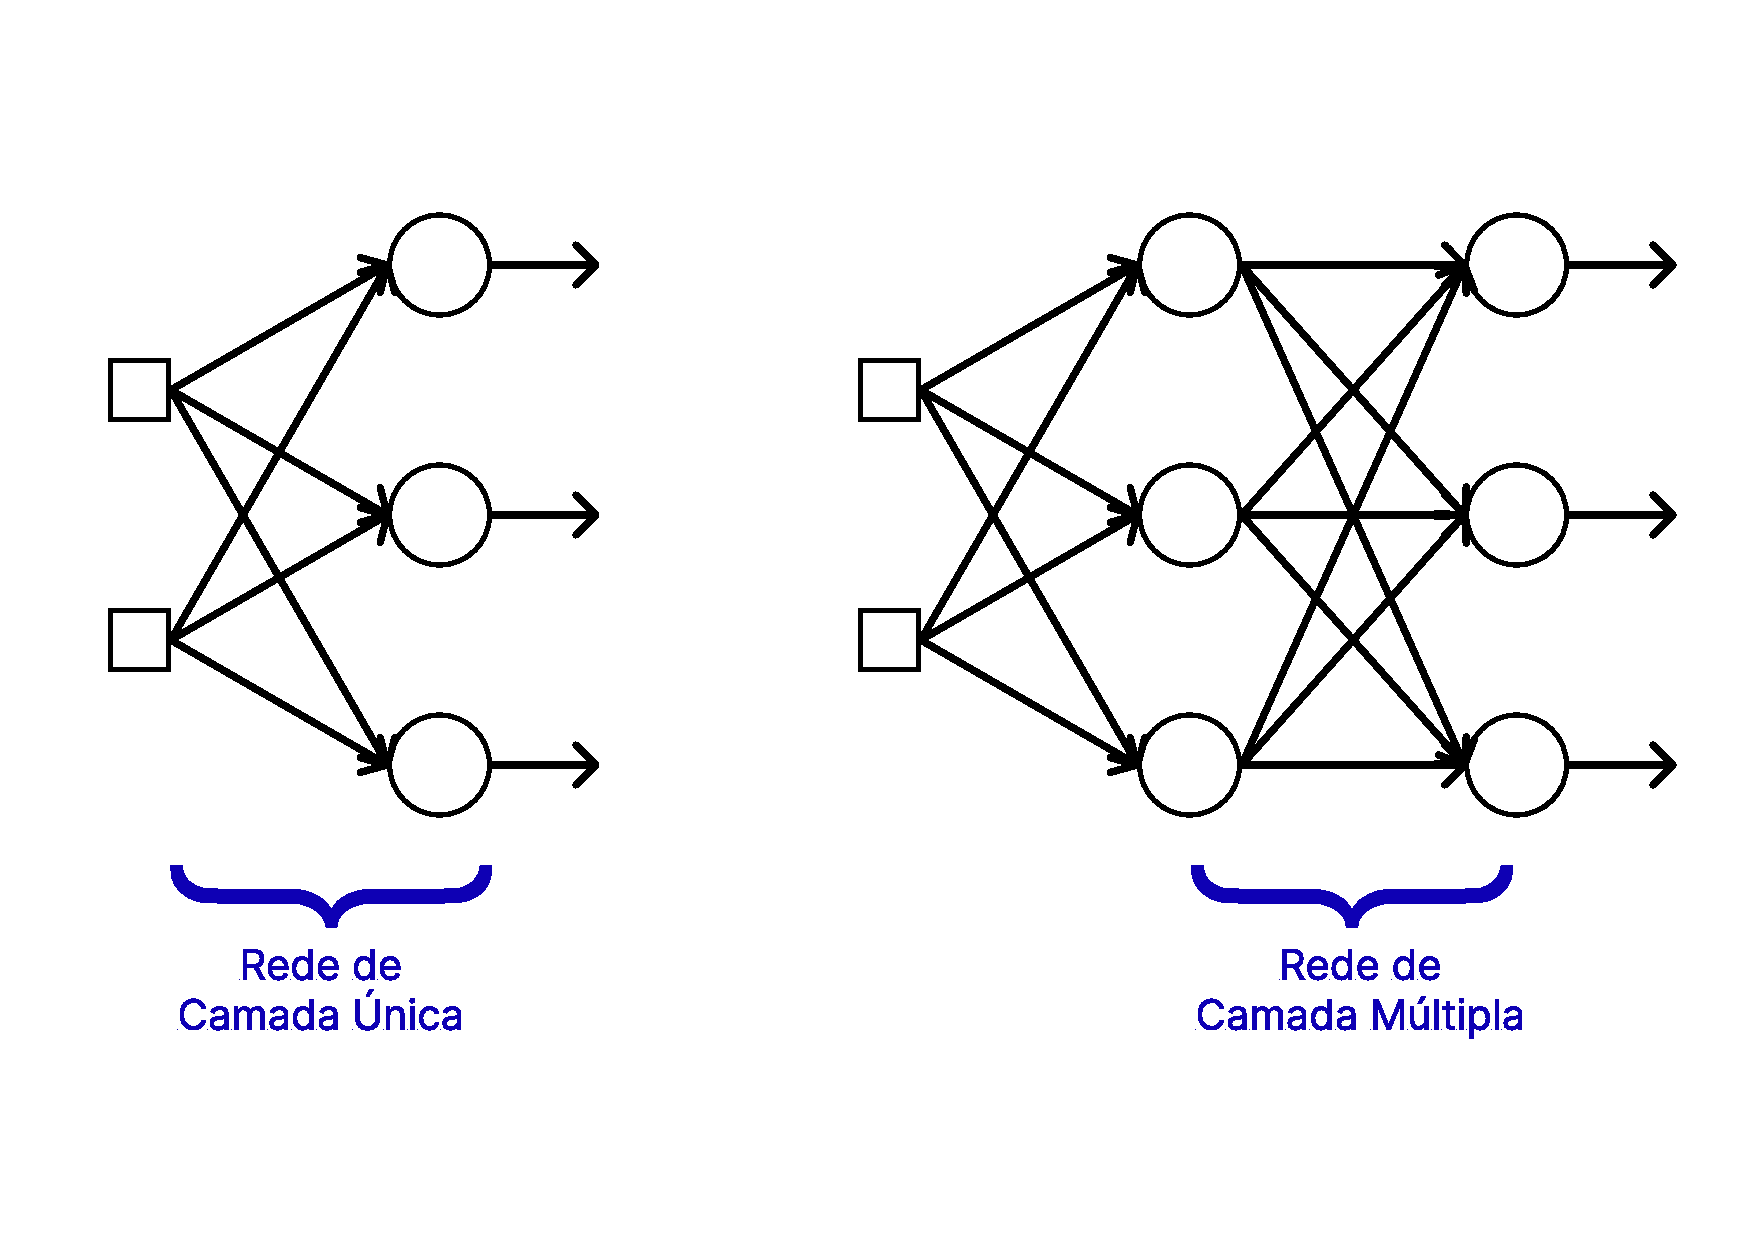
\includegraphics[scale=0.25]{figuras/network_layers.pdf}
		    \caption{Rede Camada Única e Múltipla \citep[adaptado de][]{haykin2009}}
	    \end{figure}
    \end{frame}

    \begin{frame}{RNN - Redes Neurais Recorrentes}
        \begin{itemize}
            \item Redes neurais recorrentes (RNNs) são um tipo de redes neurais criadas para processar séries temporais e outros tipos de dados sequenciais \citep{fan2021}.
            \item Uma RNN pode consistir de uma única camada de neurônios, com cada neurônio alimentando seu sinal de volta para as entradas de todos os outros neurônios \citep{haykin2009}.
        \end{itemize}
    \end{frame}
    
    \begin{frame}{RNN - Redes Neurais Recorrentes}
        \begin{figure}
            \centering
            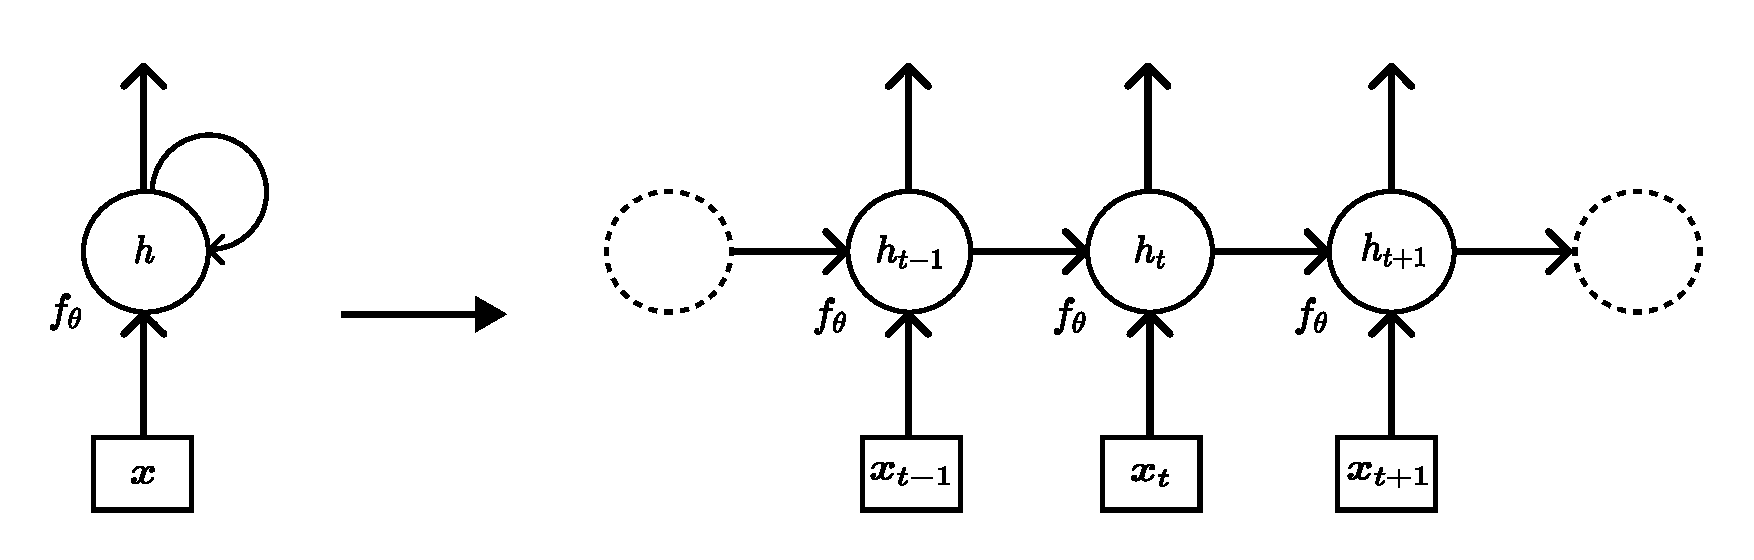
\includegraphics[scale=0.35]{figuras/rnn_hidden_state.pdf}
	        \caption{Diagrama de uma RNN \textit{Vanilla} \citep[adaptado de][]{goodfellow2016, kamath2019}}
        \end{figure}
    \end{frame}
    
    \begin{frame}{LSTM - \textit{Long Short-Term Memory}}
        \begin{itemize}
            \justifying
            \item De acordo com \citet{goodfellow2016}, as LSTM fazem parte de uma classe de modelos chamada de RNN fechadas (\textit{gated RNN}).
            \item Os portões (\textit{gates}), que também são camadas da rede neural, controlam o fluxo de informação, mantendo ou descartando o estado oculto $\bs{h}_{t}$ a cada passo temporal \citep{kamath2019}.
        \end{itemize}  
    \end{frame}
    
    \begin{frame}{LSTM - \textit{Long Short-Term Memory}}
       \begin{figure}
            \centering
            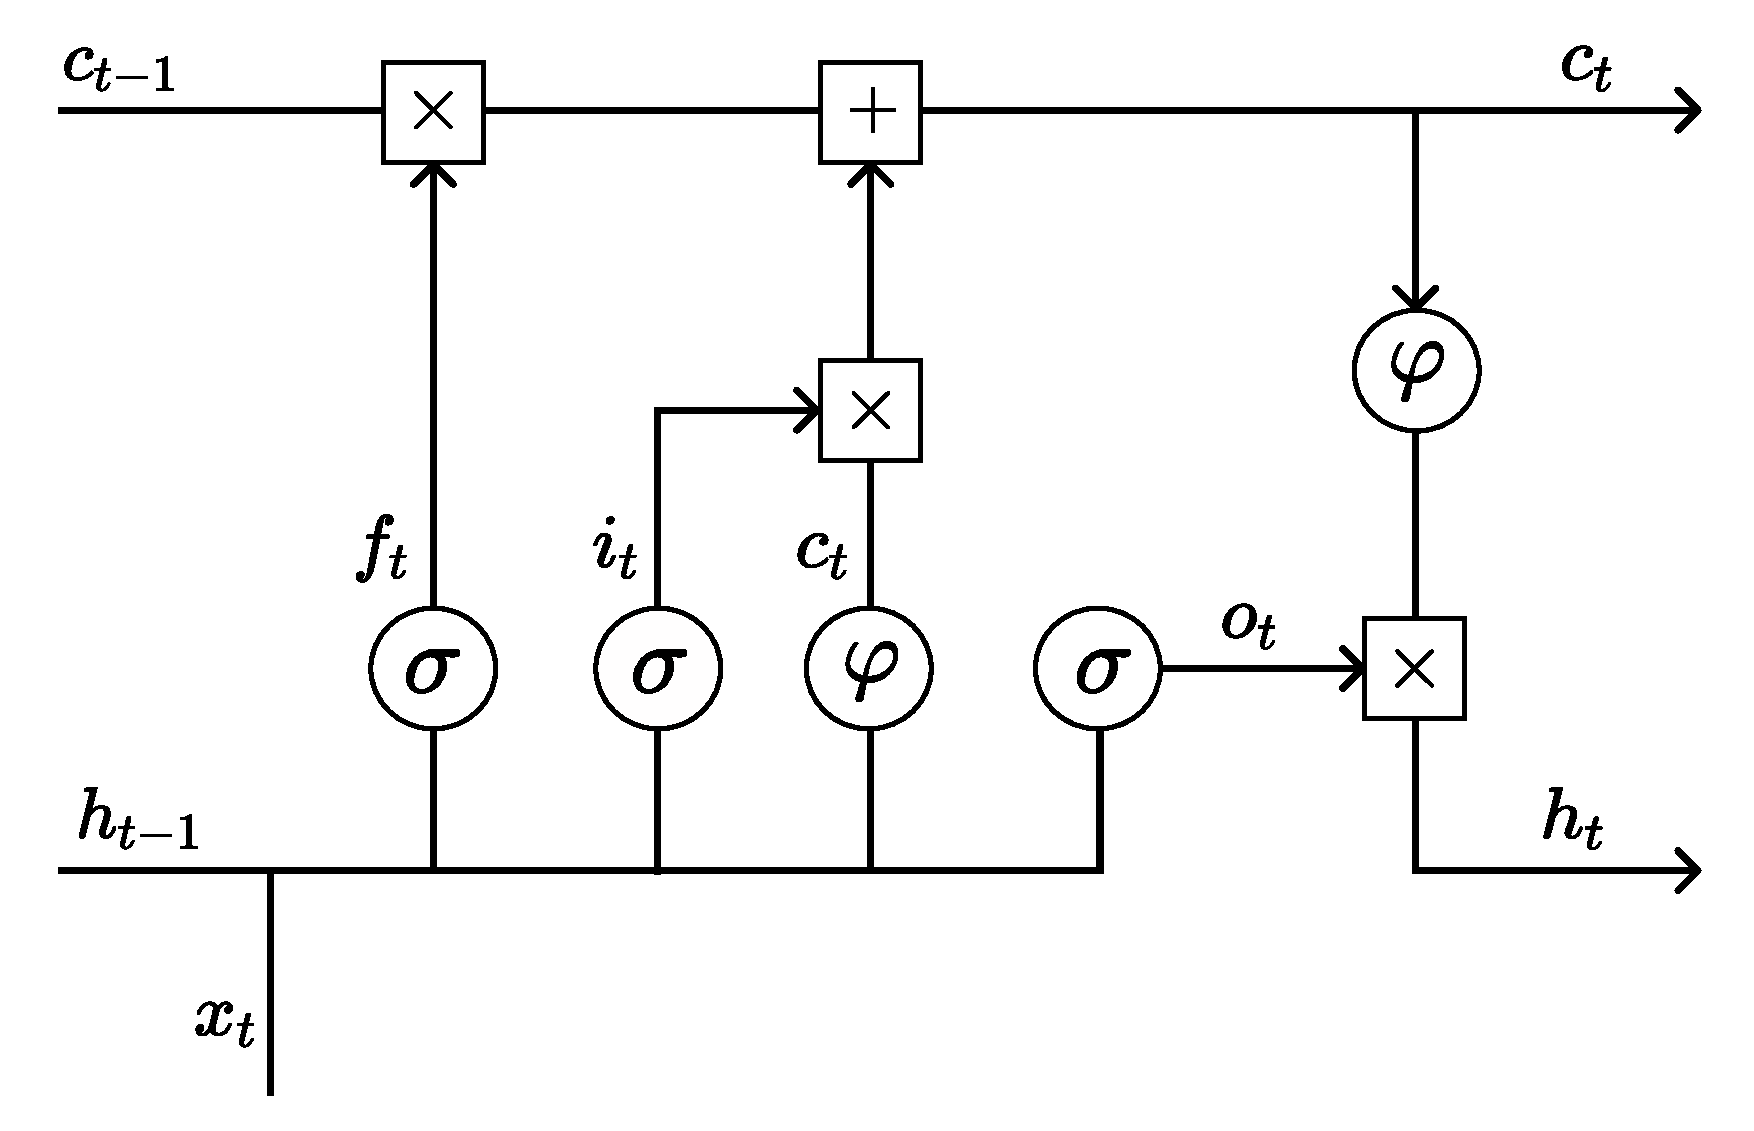
\includegraphics[scale=0.25]{figuras/lstm_cell.pdf}
	        \caption{Diagrama de uma LSTM. Considere $\sigma$ como a função de ativação \textit{logit} \citep[adaptado de][]{kamath2019}.}
        \end{figure}
    \end{frame}

    \begin{frame}{RNA - Ajuste}
        Algoritmos de aprendizagem de máquina, usualmente, envolvem alguma parte de otimização, referindo-se a minimizar (ou maximizar) uma função $f(x)$. Tal função pode ser chamada de \textbf{função custo} (\textit{cost function}) ou de \textbf{função perda} (\textit{loss function}). 
        
        bla bla bla
    \end{frame}

    \begin{frame}{PLN - Processamento de Linguagem Natural}
        Processamento de Linguagem Natural (PLN), também conhecida como Linguística Computacional, foca na aplicação de métodos quantitativos e estatísticos para entender como seres humanos modelam linguagem, bem como abordagens computacionais para responder perguntas linguísticas. Ou seja, é a aplicação de métodos computacionais para modelar e extrair informações da linguagem humana \citep{kamath2019}.
    \end{frame}
    
    \begin{frame}{PLN - Corpus}
        Um \textit{corpus} (plural \textit{corpora}) é uma coleção de material textual (seja em um único documento ou uma coleção de documentos) construído de acordo com algum critério. Esse material é constituído com ao menos uma linguagem escrita (representação via símbolos de uma linguagem falada ou gestual).
    \end{frame}
    
    \begin{frame}{PLN - Expressões Regulares}
        Expressões Regulares são particularmente úteis para pesquisar em textos, localizando determinados padrões em um \textit{corpus}. \citet{jurafsky2021} comentam que, formalmente, uma expressão regular é uma notação algébrica utilizada para caracterizar um conjunto de \textit{strings}.
    \end{frame}
    
    \begin{frame}{PLN - Tokenização}
        Tokenização é o processo computacional de segmentar texto em unidades denominadas \textit{tokens}, podendo ser palavras, números ou sinais de pontuação. Em seu processo mais simples, tokenização pode ser realizada ao separar texto por espaços em branco, induzindo um vocabulário ou um dicionário \citep{kamath2019, jurafsky2021}.
    \end{frame}
    
    \begin{frame}{PLN - Modelo de Linguagem}
        Um modelo estatístico de linguagem é aquele que atribui probabilidades para uma sequência de \textit{tokens}. Por exemplo, pode-se determinar a probabilidade de uma determinada sequência por meio da probabilidade de cada \textit{token} disponível nos \textit{tokens} anteriores. Dentre suas aplicações, tem-se reconhecimento de fala, tradução automática, marcação de parte da fala (\textit{part-of-speech tagging}), reconhecimento de manuscrito, recuperação de informação, entre outras \citep{kamath2019, jurafsky2021}.
    \end{frame}

    \begin{frame}{PLN - Avaliação Intrínseca e Extrínseca}
        Existem dois tipos de avaliação de um modelo de linguagem: extrínseca e intrínseca. Uma avaliação \textbf{extrínseca} envolve encapsular o modelo em uma aplicação e medir se houve melhorias. Por exemplo, em um contexto de reconhecimento de fala, o texto transcrito seria comparado com o discurso realizado. Apesar da avaliação extrínseca verificar qual ajuste melhora o desempenho do modelo, desenvolver um sistema completo para tal objetivo é usualmente caro, afetando sua viabilidade. Uma alternativa é a avaliação \textbf{intrínseca}, que consiste em utilizar uma métrica objetiva para mensurar as potenciais melhorias do modelo de linguagem. Basicamente, é um tipo de avaliação que mede a qualidade de um modelo independentemente de sua aplicação. No entanto, uma melhora na métrica intrínseca não necessariamente implica em uma melhora na avaliação extrínseca.
    \end{frame}
    
    \begin{frame}{PLN - Entropia}
        bla bla bla
    \end{frame}

\section{Modelagem}
    \begin{frame}{mod1}
        bla bla bla
    \end{frame}

    \begin{frame}{mod2}
        bla bla bla
    \end{frame}

    \begin{frame}{mod3}
        bla bla bla
    \end{frame}


\section{Resultados}
    \begin{frame}{rslt1}
        \citep{agarwala2017}
    \end{frame}
    
    \begin{frame}{rslt2}
        bla bla bla
    \end{frame}
    
    \begin{frame}{rslt3}
        bla bla bla
    \end{frame}
    
    \begin{frame}{rslt4}
        bla bla bla
    \end{frame}


\section{Considerações Finais}
    \begin{frame}{end1}
        bla bla bla
    \end{frame}
    
    \begin{frame}{end2}
        bla bla bla
    \end{frame}

%
    \begin{frame}[allowframebreaks]
        \frametitle{References}
        \bibliographystyle{apalike}
        \bibliography{biblio}
        
    \end{frame}


\end{document}